% import
\documentclass[conference]{IEEEtran}
\IEEEoverridecommandlockouts
\usepackage{cite}
\usepackage{amsmath,amssymb,amsfonts}
\usepackage{algorithmic}
\usepackage{graphicx}
\usepackage{textcomp}
\usepackage{xcolor}
\usepackage{diagbox}
\def\BibTeX{{\rm B\kern-.05em{\sc i\kern-.025em b}\kern-.08em
    T\kern-.1667em\lower.7ex\hbox{E}\kern-.125emX}}

% document start
\begin{document}

\title{Searching Algorithm for Match Mapping in Kidney Exchange Program}

% author
\author{\IEEEauthorblockN{Fazat Nur Azizah}
\IEEEauthorblockA{fazat@informatika.org}
\and
\IEEEauthorblockN{Ardian Umam}
\IEEEauthorblockA{ardian@informatika.org}
\and
\IEEEauthorblockN{Leonardo}
\IEEEauthorblockA{13517048@std.stei.itb.ac.id}
}

\maketitle

\begin{abstract}
Before kidney transplant is performed, the kidney donor and the kidney recipient must
be a compatible pair. In reality, it's not uncommon that incompatibility occurs between the donor-recipient pair.
To solve this problem, Kidney Exchange Program was created so that an incompatible pair can exchange the kidney
to another incompatible pair, making cross donation easier. But to search for the optimal match map from incompatible
pairs pool is not an easy task. Match map searching algorithm is an algorithm created for this task. Edmond's
Algorithm, the existing algorithm, is suboptimal because it closes the possibiliy of three or more-way exchanges.
Therefore, in this paper, by modifying existing two-way match map searching algorithms, \textit{N}-way match
map searching algorithm is implemented. Based on the test results, using 3000 incompatible pairs data, it is
proven that \textit{N}-way match map searching algorithm is superior in terms of matching efficiency compared to
the two-way match map searching algorithm. The increase in matching efficiency obtained on average reaches 7.75\%
in comparison to the matching efficiency obtained by Edmond's Algorithm. 
\end{abstract}

\begin{IEEEkeywords}
kidney transplantation, kidney exchange, match map searching algorithm
\end{IEEEkeywords}

\section{Introduction}
Every year, in Indonesia alone, there are more than 100,000 patients with kidney needs. But among
those patients, only about 20\% can get a kidney transplantation \cite{wiradarma}. There are many types
of problems that leads to this condition, for example financial problems, public opinions, and the most
common, kidney availability.
This availability problem arises because many criteria must be met before kidney transplant can be
performed \cite{wiradarma}. The donor needs to have a healthy kidney, matching blood type, and no blood-borne
diseases. Also, the patient's immune system must be able to accept the donor's kidney without killing it.

\subsection{Kidney Transplant Prerequisites}
\begin{table}[htbp]
    \caption{Blood Type Compatibility between Patient and Donor \cite{raja}}
    \begin{center}
    \def\arraystretch{1.5}
    \begin{tabular}{|c|c|c|c|c|}
    \hline
    \backslashbox{\textbf{Recipient}}{\textbf{Donor}}&\textbf{O}&\textbf{A}&\textbf{B}&\textbf{AB} \\
    \hline
    \textbf{O}&1&0&0&0 \\
    \hline
    \textbf{A}&1&1&0&0 \\
    \hline
    \textbf{B}&1&0&1&0 \\
    \hline
    \textbf{AB}&1&1&1&1 \\
    \hline
    \end{tabular}
    \label{tab1}
    \end{center}
\end{table}

The blood type test, is performed to both the donor and the recipient. Donors can only make a
donation if one's blood type is compatible with the recipient's blood type.
In Table I, number 1 indicates compatibility and 0 indicates incompatibility. Donors with blood type
O are considered Universal Donors because they can give donors to every patients regardless of the blood
type. Recipients with blood type AB are considered a Universal Recipients because they can accept kidney
donation from every donors regardless of the blood type \cite{charge}.
The immune test is performed after the donor-recipient pair passes the blood type test \cite{adrian}. The tests
are cross match test and Human Leucocyte Antigen (HLA) test. In cross match test, donor's blood are met with
recipient's blood to see whether there is a resistance reaction from recipient's immune system. The resistance
reaction happens when the donor kidney is considered a foreign object that must be killed by recipient's
immune system \cite{aprilano}. HLA test tests the same reaction as cross match test, but donor's and recipient's
tissue cells are being used instead of blood \cite{nguyen}.
Finally, to test whether the donor has any blood-borne diseases, serology is performed \cite{aprilano}.

\subsection{Kidney Exchange Program}
Because of kidney transplant prerequisites, Kidney Exchange program named Kidney Paired Donation (KPD) was created \cite{raja}
so that an incompatible donor-recipient pair can exchange their incompatible kidney to another incompatible
pair, making cross-donation possible. The kidney exchange can be done two-way and can go up to \textit{N}-way.

\begin{figure}[h]
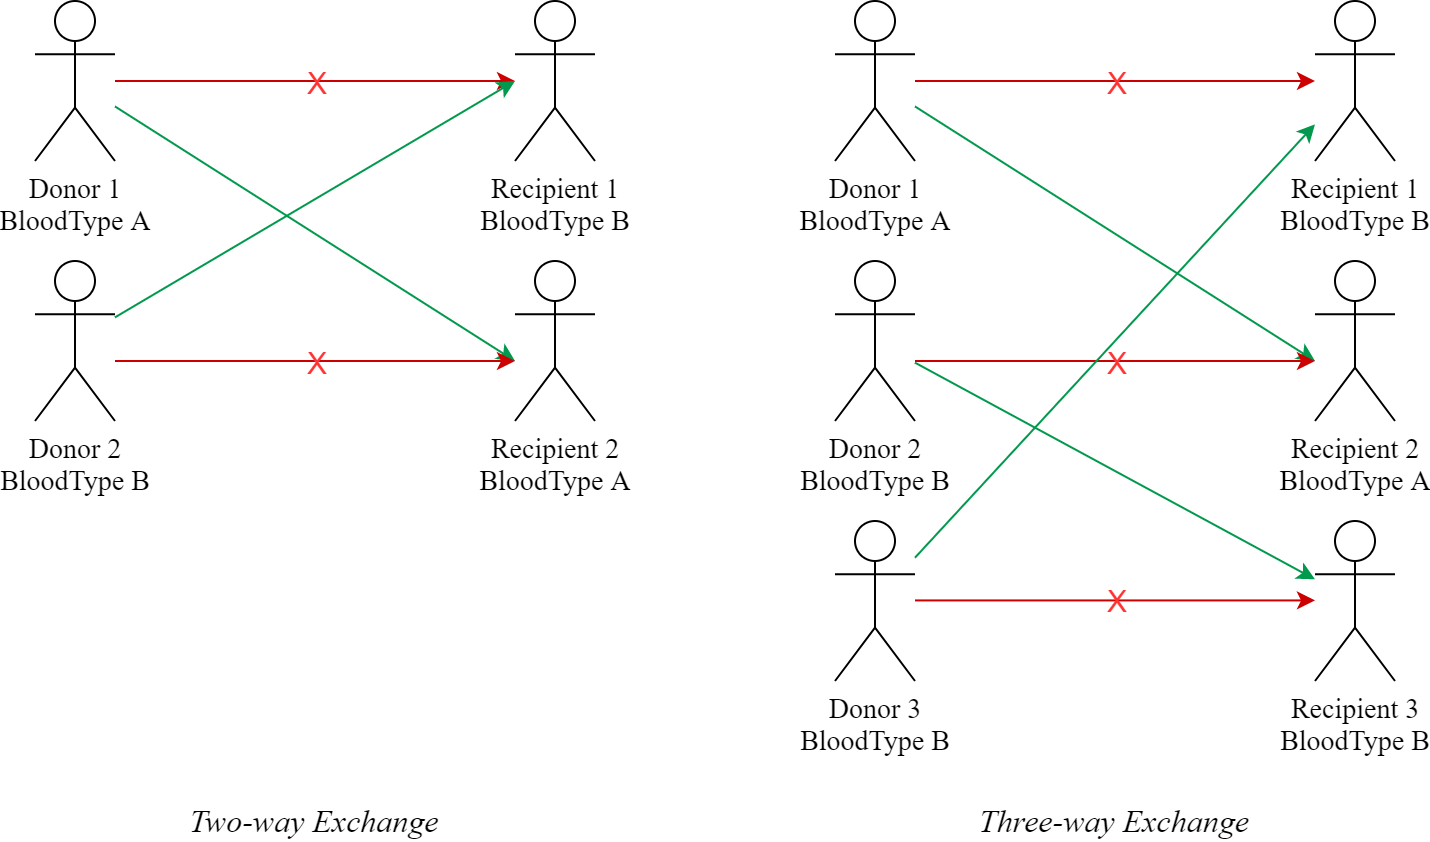
\includegraphics[width=0.5\textwidth]{images/kidney-exchange.png}
\caption{Two-way(left) and Three-way(right) Exchange in KPD program}
\end{figure}

Unfortunately, because of the large number of incompatible pairs, hospitals cannot find the optimal
matching solution for the pool of incompatible pairs. An algorithm that perform a mapping search is needed
to address this issue. One of the most known algorithm to tackle this problem is Edmond's Algorithm \cite{raja}.
In Edmond's Algorithm, the pool of incompatible pairs are represented as a graph with each node representing
an incompatible pair and each edge representing a match between two incompatible pairs. The algorithm focuses on
high priority pairs so that pairs who need a transplantation more can get an exchange first.
Another algorithm regarding this problem is First Accept Heuristic Match \cite{raja} which focuses more on the
heuristic if one registers first, then one gets an exchange first.

These algorithms are called Match Map Searching Algorithms. There are two performance metrics to evaluate these
algorithms. The first one is Matching Efficiency, which measures the number of donor-patient pairs that matched
another pair and were able to exchange divided by the total number of donor-patient pairs, represented in a percentage.
The second metric is execution time, which measures how long does the algorithm run to get the optimal match map,
usually measured in millisecond. The best match map searching algorithm is the algorithm that can produce high matching
efficiency with low execution time. Meaning that many patients can be saved as fast as possible.

As good as it looks, Edmond's Algorithm and First Accept Heuristic Match can only find two-way exchanges from the
incompatible pairs pool. Meaning these algorithms are not able find a solution with three-way exchanges or more,
closing the possibility.

\section{Methodology}
From the existing algorithms problems addressed in the previous section, match map searching algorithms that can find
\textit{N}-way exchanges from incompatible pairs pool are needed.

\subsection{Maintaining the Integrity of the Specifications}

The IEEEtran class file is used to format your paper and style the text. All margins, 
column widths, line spaces, and text fonts are prescribed; please do not 
alter them. You may note peculiarities. For example, the head margin
measures proportionately more than is customary. This measurement 
and others are deliberate, using specifications that anticipate your paper 
as one part of the entire proceedings, and not as an independent document. 
Please do not revise any of the current designations.

\section{Experiment}
Before you begin to format your paper, first write and save the content as a 
separate text file. Complete all content and organizational editing before 
formatting. Please note sections \ref{AA}--\ref{SCM} below for more information on 
proofreading, spelling and grammar.

Keep your text and graphic files separate until after the text has been 
formatted and styled. Do not number text heads---{\LaTeX} will do that 
for you.

\subsection{Abbreviations and Acronyms}\label{AA}
Define abbreviations and acronyms the first time they are used in the text, 
even after they have been defined in the abstract. Abbreviations such as 
IEEE, SI, MKS, CGS, ac, dc, and rms do not have to be defined. Do not use 
abbreviations in the title or heads unless they are unavoidable.

\subsection{Units}
\begin{itemize}
\item Use either SI (MKS) or CGS as primary units. (SI units are encouraged.) English units may be used as secondary units (in parentheses). An exception would be the use of English units as identifiers in trade, such as ``3.5-inch disk drive''.
\item Avoid combining SI and CGS units, such as current in amperes and magnetic field in oersteds. This often leads to confusion because equations do not balance dimensionally. If you must use mixed units, clearly state the units for each quantity that you use in an equation.
\item Do not mix complete spellings and abbreviations of units: ``Wb/m\textsuperscript{2}'' or ``webers per square meter'', not ``webers/m\textsuperscript{2}''. Spell out units when they appear in text: ``. . . a few henries'', not ``. . . a few H''.
\item Use a zero before decimal points: ``0.25'', not ``.25''. Use ``cm\textsuperscript{3}'', not ``cc''.)
\end{itemize}

\subsection{Equations}
Number equations consecutively. To make your 
equations more compact, you may use the solidus (~/~), the exp function, or 
appropriate exponents. Italicize Roman symbols for quantities and variables, 
but not Greek symbols. Use a long dash rather than a hyphen for a minus 
sign. Punctuate equations with commas or periods when they are part of a 
sentence, as in:
\begin{equation}
a+b=\gamma\label{eq}
\end{equation}

Be sure that the 
symbols in your equation have been defined before or immediately following 
the equation. Use ``\eqref{eq}'', not ``Eq.~\eqref{eq}'' or ``equation \eqref{eq}'', except at 
the beginning of a sentence: ``Equation \eqref{eq} is . . .''

\subsection{\LaTeX-Specific Advice}

Please use ``soft'' (e.g., \verb|\eqref{Eq}|) cross references instead
of ``hard'' references (e.g., \verb|(1)|). That will make it possible
to combine sections, add equations, or change the order of figures or
citations without having to go through the file line by line.

Please don't use the \verb|{eqnarray}| equation environment. Use
\verb|{align}| or \verb|{IEEEeqnarray}| instead. The \verb|{eqnarray}|
environment leaves unsightly spaces around relation symbols.

Please note that the \verb|{subequations}| environment in {\LaTeX}
will increment the main equation counter even when there are no
equation numbers displayed. If you forget that, you might write an
article in which the equation numbers skip from (17) to (20), causing
the copy editors to wonder if you've discovered a new method of
counting.

{\BibTeX} does not work by magic. It doesn't get the bibliographic
data from thin air but from .bib files. If you use {\BibTeX} to produce a
bibliography you must send the .bib files. 

{\LaTeX} can't read your mind. If you assign the same label to a
subsubsection and a table, you might find that Table I has been cross
referenced as Table IV-B3. 

{\LaTeX} does not have precognitive abilities. If you put a
\verb|\label| command before the command that updates the counter it's
supposed to be using, the label will pick up the last counter to be
cross referenced instead. In particular, a \verb|\label| command
should not go before the caption of a figure or a table.

Do not use \verb|\nonumber| inside the \verb|{array}| environment. It
will not stop equation numbers inside \verb|{array}| (there won't be
any anyway) and it might stop a wanted equation number in the
surrounding equation.

\subsection{Some Common Mistakes}\label{SCM}
\begin{itemize}
\item The word ``data'' is plural, not singular.
\item The subscript for the permeability of vacuum $\mu_{0}$, and other common scientific constants, is zero with subscript formatting, not a lowercase letter ``o''.
\item In American English, commas, semicolons, periods, question and exclamation marks are located within quotation marks only when a complete thought or name is cited, such as a title or full quotation. When quotation marks are used, instead of a bold or italic typeface, to highlight a word or phrase, punctuation should appear outside of the quotation marks. A parenthetical phrase or statement at the end of a sentence is punctuated outside of the closing parenthesis (like this). (A parenthetical sentence is punctuated within the parentheses.)
\item A graph within a graph is an ``inset'', not an ``insert''. The word alternatively is preferred to the word ``alternately'' (unless you really mean something that alternates).
\item Do not use the word ``essentially'' to mean ``approximately'' or ``effectively''.
\item In your paper title, if the words ``that uses'' can accurately replace the word ``using'', capitalize the ``u''; if not, keep using lower-cased.
\item Be aware of the different meanings of the homophones ``affect'' and ``effect'', ``complement'' and ``compliment'', ``discreet'' and ``discrete'', ``principal'' and ``principle''.
\item Do not confuse ``imply'' and ``infer''.
\item The prefix ``non'' is not a word; it should be joined to the word it modifies, usually without a hyphen.
\item There is no period after the ``et'' in the Latin abbreviation ``et al.''.
\item The abbreviation ``i.e.'' means ``that is'', and the abbreviation ``e.g.'' means ``for example''.
\end{itemize}
An excellent style manual for science writers is \cite{b7}.

\subsection{Authors and Affiliations}
\textbf{The class file is designed for, but not limited to, six authors.} A 
minimum of one author is required for all conference articles. Author names 
should be listed starting from left to right and then moving down to the 
next line. This is the author sequence that will be used in future citations 
and by indexing services. Names should not be listed in columns nor group by 
affiliation. Please keep your affiliations as succinct as possible (for 
example, do not differentiate among departments of the same organization).

\subsection{Identify the Headings}
Headings, or heads, are organizational devices that guide the reader through 
your paper. There are two types: component heads and text heads.

Component heads identify the different components of your paper and are not 
topically subordinate to each other. Examples include Acknowledgments and 
References and, for these, the correct style to use is ``Heading 5''. Use 
``figure caption'' for your Figure captions, and ``table head'' for your 
table title. Run-in heads, such as ``Abstract'', will require you to apply a 
style (in this case, italic) in addition to the style provided by the drop 
down menu to differentiate the head from the text.

Text heads organize the topics on a relational, hierarchical basis. For 
example, the paper title is the primary text head because all subsequent 
material relates and elaborates on this one topic. If there are two or more 
sub-topics, the next level head (uppercase Roman numerals) should be used 
and, conversely, if there are not at least two sub-topics, then no subheads 
should be introduced.

\subsection{Figures and Tables}
\paragraph{Positioning Figures and Tables} Place figures and tables at the top and 
bottom of columns. Avoid placing them in the middle of columns. Large 
figures and tables may span across both columns. Figure captions should be 
below the figures; table heads should appear above the tables. Insert 
figures and tables after they are cited in the text. Use the abbreviation,
even at the beginning of a sentence.

\begin{table}[htbp]
\caption{Table Type Styles}
\begin{center}
\begin{tabular}{|c|c|c|c|}
\hline
\textbf{Table}&\multicolumn{3}{|c|}{\textbf{Table Column Head}} \\
\cline{2-4} 
\textbf{Head} & \textbf{\textit{Table column subhead}}& \textbf{\textit{Subhead}}& \textbf{\textit{Subhead}} \\
\hline
copy& More table copy$^{\mathrm{a}}$& &  \\
\hline
\multicolumn{4}{l}{$^{\mathrm{a}}$Sample of a Table footnote.}
\end{tabular}
\label{tab2}
\end{center}
\end{table}

Figure Labels: Use 8 point Times New Roman for Figure labels. Use words 
rather than symbols or abbreviations when writing Figure axis labels to 
avoid confusing the reader. As an example, write the quantity 
``Magnetization'', or ``Magnetization, M'', not just ``M''. If including 
units in the label, present them within parentheses. Do not label axes only 
with units. In the example, write ``Magnetization (A/m)'' or ``Magnetization 
\{A[m(1)]\}'', not just ``A/m''. Do not label axes with a ratio of 
quantities and units. For example, write ``Temperature (K)'', not 
``Temperature/K''.

\section{Results and Analysis}
ababwa

\section{Related Work}
this is still a template

\section{Conclusion}
ababwa

\section*{Acknowledgment}

The preferred spelling of the word ``acknowledgment'' in America is without 
an ``e'' after the ``g''. Avoid the stilted expression ``one of us (R. B. 
G.) thanks $\ldots$''. Instead, try ``R. B. G. thanks$\ldots$''. Put sponsor 
acknowledgments in the unnumbered footnote on the first page.

\section*{References}

Please number citations consecutively within brackets \cite{b1}. The 
sentence punctuation follows the bracket \cite{b2}. Refer simply to the reference 
number, as in \cite{b3}---do not use ``Ref. \cite{b3}'' or ``reference \cite{b3}'' except at 
the beginning of a sentence: ``Reference \cite{b3} was the first $\ldots$''

Number footnotes separately in superscripts. Place the actual footnote at 
the bottom of the column in which it was cited. Do not put footnotes in the 
abstract or reference list. Use letters for table footnotes.

Unless there are six authors or more give all authors' names; do not use 
``et al.''. Papers that have not been published, even if they have been 
submitted for publication, should be cited as ``unpublished'' \cite{b4}. Papers 
that have been accepted for publication should be cited as ``in press'' \cite{b5}. 
Capitalize only the first word in a paper title, except for proper nouns and 
element symbols.

For papers published in translation journals, please give the English 
citation first, followed by the original foreign-language citation \cite{b6}.

\begin{thebibliography}{00}
\bibitem{wiradarma} Wiradarma, K. (2016, February 3). Transplantasi Ginjal di Indonesia: Pencapaian dan Hambatannya. Retrieved from klikdokter.com: https://www.klikdokter.com/info-sehat/read/2697086/transplantasi-ginjal-di-indonesia-pencapaian-dan-hambatannya
\bibitem{raja} Raja, S., S., P. D., K., S. R. (2011). Web Based Decision Support System for Kidney. International Journal of Computer Applications (0975 – 8887), 9.
\bibitem{charge} Chargé, S., Hodgkinson, K. (2017, January). Blood: the basics. Retrieved from profedu.blood.ca/: https://profedu.blood.ca/en/transfusion/publications/blood-basics.
\bibitem{adrian} Adrian, K. (2020, May 17). Berbagai Persiapan Donor Ginjal yang Perlu Anda Ketahui. Retrieved from alodokter.com: https://www.alodokter.com/hal-hal-yang-harus-diperhatikan-sebelum-melakukan-donor-ginjal
\bibitem{aprilano} Aprilano, W. D. (2021, January 20). Teknik Transplantasi Ginjal. Retrieved from alomedika.com: https://www.alomedika.com/tindakan-medis/transplantasi/transplantasi-ginjal/teknik
\bibitem{nguyen} Nguyen, H. D., Williams, R. L., Wong, G., Lim, W. H. (2013, February 13). The Evolution of HLA-Matching in Kidney Transplantation. Retrieved from intechopen.com: https://www.intechopen.com/books/current-issues-and-future-direction-in-kidney-transplantation/the-evolution-of-hla-matching-in-kidney-transplantation
\bibitem{mehta} Mehta, D. (2020, May 27). Detect Cycle in a Directed Graph. Retrieved from geeksforgeeks.org: https://www.geeksforgeeks.org/detect-cycle-in-a-graph/
\bibitem{roth2005} Roth, A. E., Sonmez, T., Unver, M. U. (2005). Kidney Exchange. Quarterly Journal of Economics, 32.
\bibitem{roth2006} Roth, A. E., Sonmez, T., Unver, M. U., Delmonico, F. L., Saidman, S. L. (2006, September 18). Utilizing List Exchange and Nondirected Donation through ‘Chain’ Paired Kidney Donations. Retrieved from onlinelibrary.wiley.com: https://onlinelibrary.wiley.com/doi/full/10.1111/j.1600-6143.2006.01515.x
\bibitem{sedgewick} Sedgewick, R., Wayne, K. (2020). Directed Graphs. In R. Sedgewick, K. Wayne, Algorithms, 4th Edition (p. 955). New Jersey: Princeton University.
\bibitem{tullis} Tullis, T., Albert, B. (2013, June 3). Performance Metrics. Retrieved from sciencedirect.com: https://www.sciencedirect.com/science/article/pii/B9780124157811000042
\end{thebibliography}

\end{document}
